\documentclass[10pt,t]{beamer}

\usepackage[utf8]{inputenc}
\usepackage[T1]{fontenc}
\usepackage{graphicx}
\usepackage{grffile}
\usepackage{longtable}
\usepackage{wrapfig}
\usepackage{rotating}
\usepackage[normalem]{ulem}
\usepackage{amsmath}
\usepackage{textcomp}
\usepackage{amssymb}
\usepackage{capt-of}
\usepackage{hyperref}

%\newcommand{\nitrous}{N$_2$O\xspace}
%\newcommand{\ozone}{O$_3$\xspace}

\input beamer_setup

\usetheme{default}
% ---------------------------------------------------------------------
% ---------------------------------------------------------------------
\begin{document}

\title[]{15 years of Longwave Flux Trends : \newline
  Roles of CO2, WV, Temperature and clouds, \newline
  using ERA and AIRS data}
\author{Sergio DeSouza-Machado, Larrabee Strow}
\institute{Department of Physics, JCET\\
  University of Maryland Baltimore County (UMBC)}
\date{October 2, 2018}
% ---------------------------------------------------------------------
% ---------------------------------------------------------------------
\begin{frame}
  \titlepage
\end{frame}
% ---------------------------------------------------------------------
\begin{frame}
  \frametitle{Overview}
  \begin{itemize}
  \item CERES can produce total OLR or window region OLR
  \item AIRS spans much of the IR, and has information about clouds, gases and temperatures
    \begin{itemize}    
    \item use LBL code (radiance/flux; slow) or RRTM (flux; fast)
    \item use TwoSlab fluxes in RRTM, likely use MRO clouds in the future
    \item \textcolor{red}{Larrabee has proposed L3 climate (trending) products from AIRS,
          this is our first use of OLR spectral fluxes as product to study climate change}
    \end{itemize}
  \item Talk focuses on contribution of various components to OLR flux changes using
    \begin{itemize}
    \item ERA fields, averaged over latbins (cloud profiles turned to TwoSlabs) \textcolor{blue}{not good enough because of ERA clouds}
    \item Our retrieved thermodynamic and cloud rates (see 3.20 pm talk by Larrabee Strow "Level 3
      AIRS/CrIS/IASI Anomalies and Trends Derived from Radiance Trends"
    \end{itemize}
  \item Antartic Fluxes "Unmasking the negative greenhouse effect over the Antarctic Plateau" by Seijas, Taylor, Cai, \emph{Nature 2018}    
  \end{itemize}
\end{frame}
% ---------------------------------------------------------------------
\section{General idea}
% ---------------------------------------------------------------------
\begin{frame}
  \frametitle{Background}
  \begin{itemize}
  \item If there was no atmosphere, then surface heated by sun (or eg nuclear energy within)
  \item Power radiated out to space would simply be $P/A = OLR = \sigma T_{surf}^4$ 
  \item However there are clouds and atmospheric gases, transporting heat and moisture globally
  \item \textcolor{blue}{\cd 15 \um band (Planck peak), BT $\sim$ 250 K or less} \newline
        \textcolor{blue}{\water Far-IR  BT is also pretty low} \newline
        \textcolor{red}{Outgoing Longwave Radiation $\ll$ radiated by surface}  
  \item Rough numbers
    \begin{small}
    \begin{itemize}
    \item Tropical atmosphere $T_{surf}$ = 299.7 K, BT1231 = 296.3 K
    \item $<T_{surf}> = 285 K, <T_{UA}> = 255 K$ greenhouse effect
    \item  Incoming TOA solar = 1360 W/m2; cross section = 340 W/m2; albedo = 0.3;
        so nominally need 238 W/m2 OLR
    \end{itemize}
    \end{small}    
  \end{itemize}
\end{frame}
% ---------------------------------------------------------------------

%\begin{frame}
%  \frametitle{kCARTA TOA radiances (TRP profile)}

%  \begin{center}
%    \noindent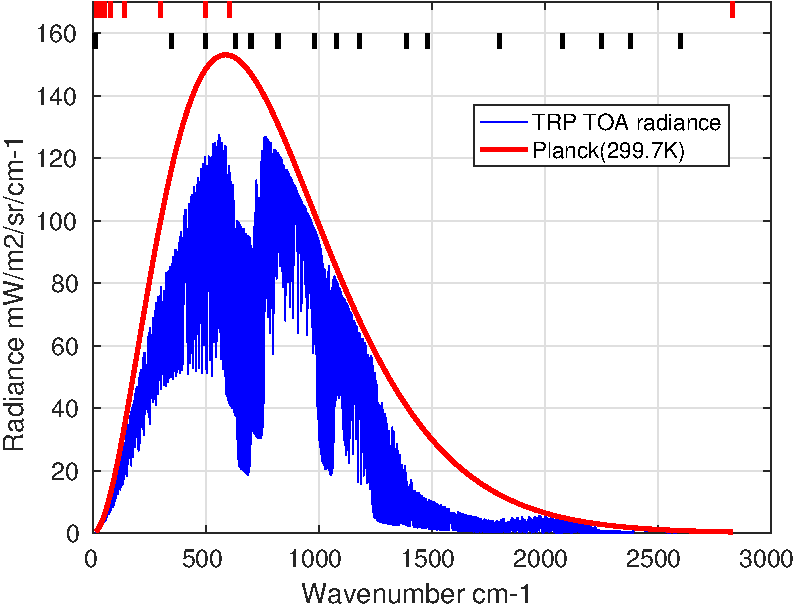
\includegraphics[width=0.625\textwidth]{Figs/generic_planckTOArads.pdf}
%  \end{center}
  
%  \begin{itemize}  
%  \item Red hashlines : kCARTA band edges
%  \item FarIR is a mix of H2004, H2008, H2012, MT-CKD 1
%  \item Cannot really do Far IR cloud calcs
%  \item so use RRTM (black hashlines : RRTM band edges)
%  \end{itemize}

%\end{frame}
% ---------------------------------------------------------------------
\begin{frame}
  \frametitle{kCARTA TOA BT (TRP profile)}

  \begin{center}
    \noindent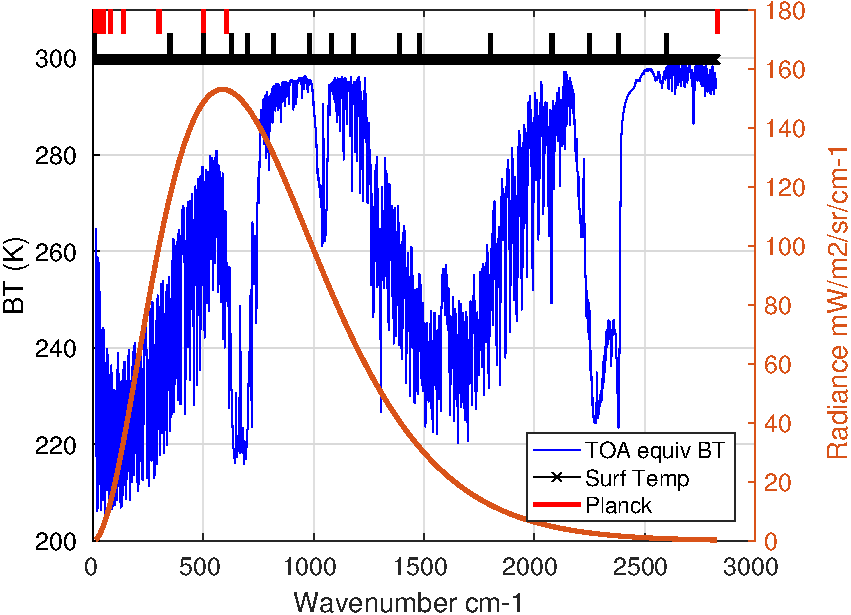
\includegraphics[width=0.75\textwidth]{Figs/generic_planckTOABT.pdf}
  \end{center}

  \begin{itemize}  
  \item Red hashlines : kCARTA band edges
  \item kCARTA liens (older spectroscopy, no cloud params in Far IR)
  \item So use RRTM (black hashlines : RRTM band edges)
  \end{itemize}

\end{frame}
% ---------------------------------------------------------------------
\begin{frame}
  \frametitle{Comparing TOA radiances and Fluxes}

  \hspace{0.50in} TOA BT1231 \hspace{1.75in} Fluxes \\
  \begin{center}
    \dlandgraph{0.48}{Figs/generic_BT1231_vs_lat.pdf}{Figs/generic_olr_vs_lat.pdf}
  \end{center}

  \begin{itemize}
  \item \textcolor{red}{RRTM : try flux calcs using TwoSlab clouds!}
  \item \begin{small}$r(\nu) = f_{ice} r_{ice}(\nu) + f_{water} r_{water}(\nu) +
    f_{overlap} r_{overlap}(\nu) + f_{clear} r_{clear}(\nu)$ \end{small}
  \item RHS : 10 W/m2 CERES/TwoSlab bias, probably not emissivity
  \end{itemize}
\end{frame}
% ---------------------------------------------------------------------
% ---------------------------------------------------------------------
\section{Obs vs Calc}
% ---------------------------------------------------------------------
% ---------------------------------------------------------------------
\begin{frame}
  \frametitle{AIRS Obs vs ERA changes : BT1231}

  Earlier Larrabee showed BT1231 Sarta TwoSlab calcs are increasing by
  0.15 K/yr in the tropics, or $\sim$ 2.25 K over 15 years \newline

  \begin{columns}
    \begin{column}{0.65\columnwidth}
      \begin{center}
        \noindent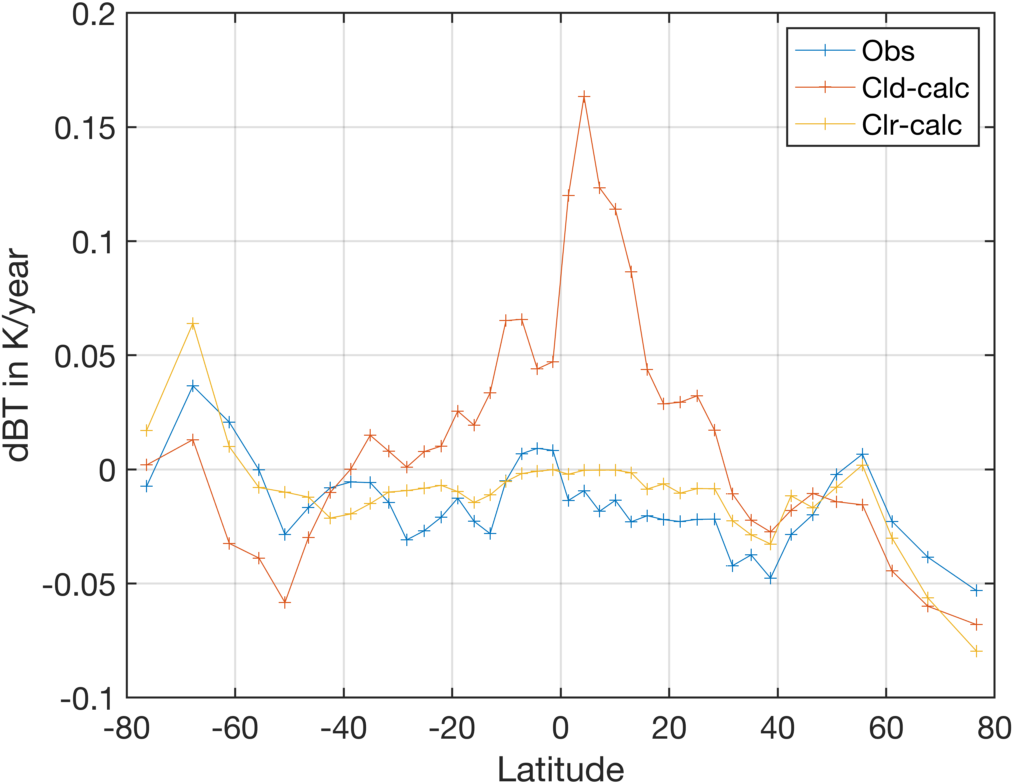
\includegraphics[width=\linewidth]{airs15year_lat_trends_900cm-1.png}
      \end{center}
    \end{column}

    \begin{column}{0.35\columnwidth}

      \vspace{0.1in}
      
      $dP = \sigma 4 T^3 dT$, with $T \sim 285 K, dT \sim 2.25 K $ $\rightarrow $
      \textcolor{red}{dP $\sim$ 11 W/m2} \newline

      That is not observed! \newline
      
      \vspace{0.1in}
      
      Can we understand where this comes from?

    \end{column}    
  \end{columns}
  
\end{frame}
% ---------------------------------------------------------------------
\begin{frame}
  \frametitle{AIRS Obs vs ERA changes : OLR}

  Take averaged profile over Year 01, all latbins, find OLR \newline
  Take averaged profile over Year 15, all latbins, find OLR \newline
  Turn on/off clouds, thermo, cloud, and CO2 changes
  
  \begin{center}
    \noindent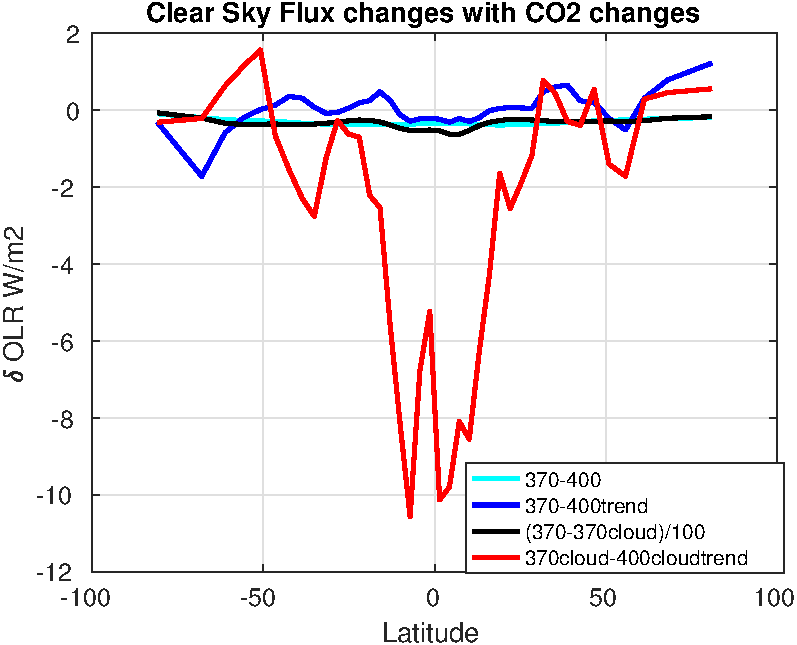
\includegraphics[width=0.625\textwidth]{Figs/deltaolr_vs_lat.pdf}
  \end{center}
\end{frame}
% ---------------------------------------------------------------------
% ---------------------------------------------------------------------
\section{Flux Jacobians}
% ---------------------------------------------------------------------
% ---------------------------------------------------------------------
\begin{frame}
  \frametitle{Flux Jacobians : Method}
  \begin{itemize}
  \item Take daily zonal averages (AIRS obs, SARTA TwoSlab calcs, ERA thermodynamics + WV,O3)
  \item Do monthly averages (giving 180 between 2002/09 to 2017/08)
  \item Compute clear sky and TwoSlab fluxes for all latitude bins/180 months
  \item Add in CO2 change $\cd(t) = 370 + 2.2/12 \delta t$ where $\delta t = (t-2002/08)$ in months
  \item Now from this do yearly averages, in particular 2002/09-2003/08 and 2016/09-2017/08
  \item Call them Y1, Y15; take the yearly averaged profiles and keep doing fluxes as one parameter
    changes, with all other parameters held constant; \textcolor{red}{these are our 15 year jacobians}
  \end{itemize}
\end{frame}
% ---------------------------------------------------------------------
\begin{frame}
  \frametitle{ERA Clear Sky Flux Jacobians: Total 15 Years}
  \vspace{-0.1in}
  \begin{center}
    \noindent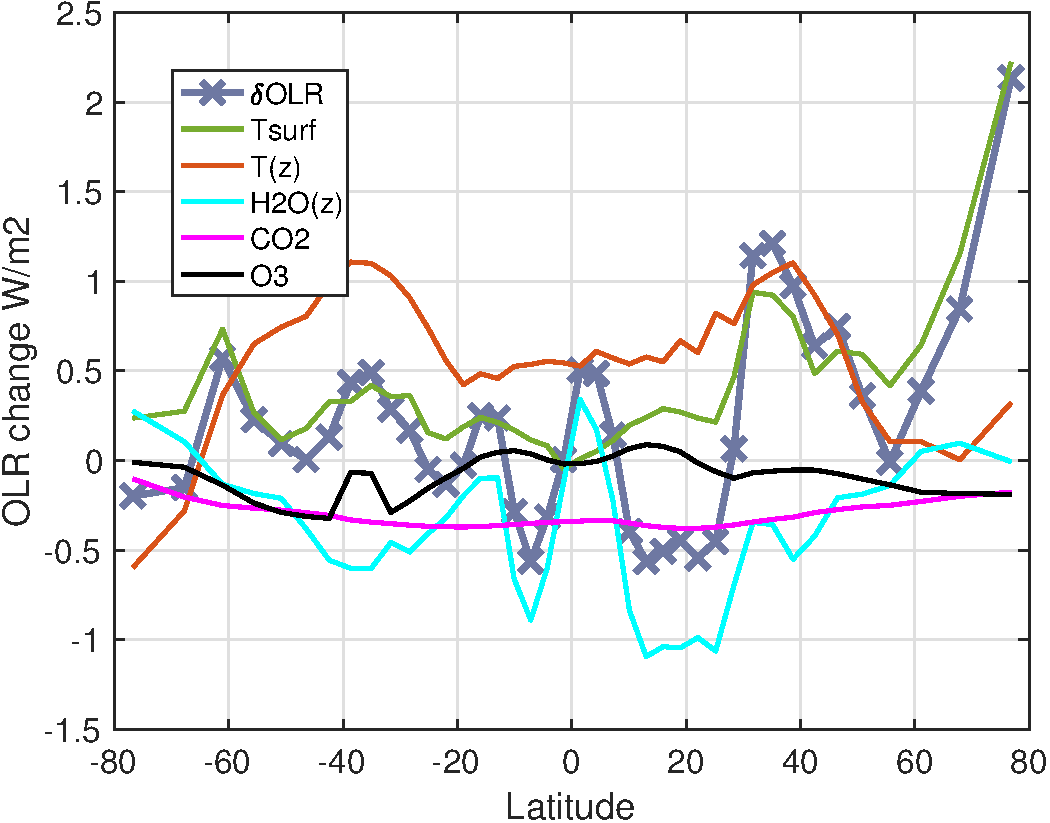
\includegraphics[width=0.75\linewidth]{clrskly_temp_gas_fluxjacs_lls.pdf}
  \end{center}
  \vspace{-0.1in}
  \begin{itemize}
  \item Lowered flux by \cd and \water
  \item Increase flux by Tsurf and T(z), \ozone small change
  \item Net change is variable except large in N. Polar regions
  \end{itemize}
\end{frame}
% ---------------------------------------------------------------------
\begin{frame}
  \frametitle{ERA All Sky Flux Jacobians : Total 15 Years}
  \vspace{-0.1in}  
  \begin{center}
    \noindent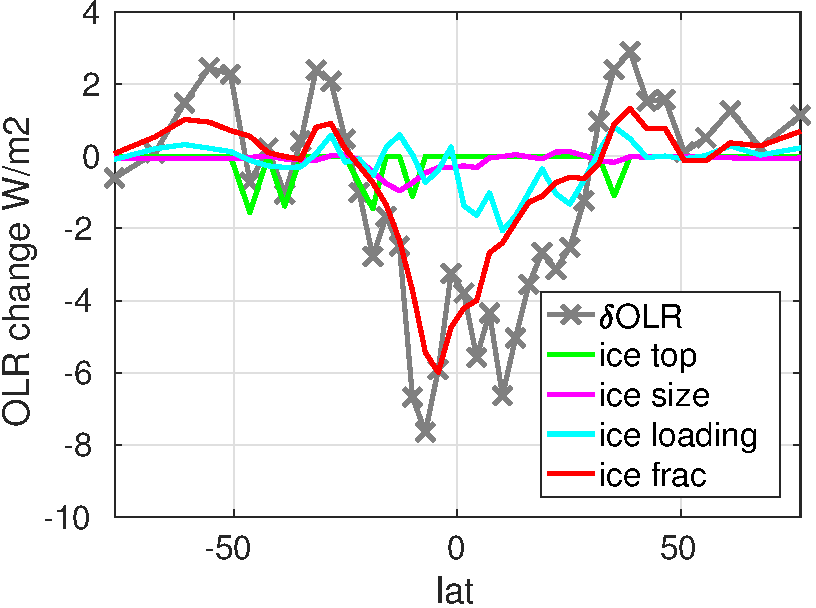
\includegraphics[width=0.75\linewidth]{Figs//allsky_cloud_fluxjacs.pdf}
  \end{center}
  \vspace{-0.1in}
  \begin{itemize}
  \item (ERA) OLR tropical decrease due to ice cloud fraction!
  \item Not shown : flux jacobians for water clouds (typically much smaller than cirrus flux jacs)
  \end{itemize}
  
  
\end{frame}
% ---------------------------------------------------------------------
% ---------------------------------------------------------------------
\section{Flux Changes Using UMBC Spectral Rates Retrievals}
% ---------------------------------------------------------------------
% ---------------------------------------------------------------------
\begin{frame}
  \frametitle{\textcolor{red}{\bf Comparison to CERES L3 rates}}
  Use Larrabee's spectral rate retrievals (cloud/thermodynamic) from previous talk;
  plug in CO2 changes over 15 years (2.2 ppmv/yr) and run through RRTM  
  \begin{center}
    \noindent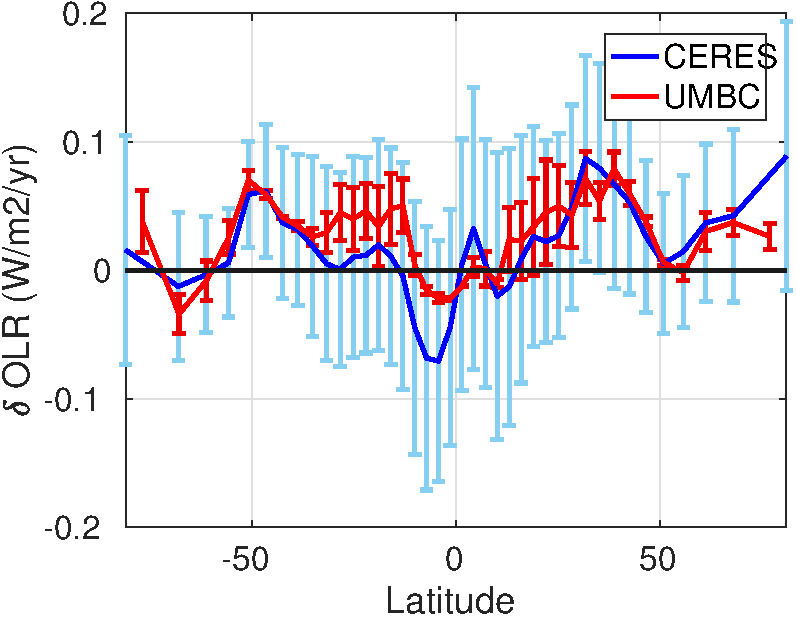
\includegraphics[width=0.625\linewidth]{Figs/umbc_vs_ceres_fluxrates.pdf}
  \end{center}
 Errorbars : TBD for next AIRS STM
\end{frame}

\begin{frame}
  \frametitle{Flux Changes by RRTM bands}
  Larrabee ran off spectral rates and OEM retrievals; enter resulting cloud and thermodynamic trends into RRTM \newline
  Red/Yellow means MORE flux (W/m2) in 2017/2018 \newline
  \begin{center}
    \noindent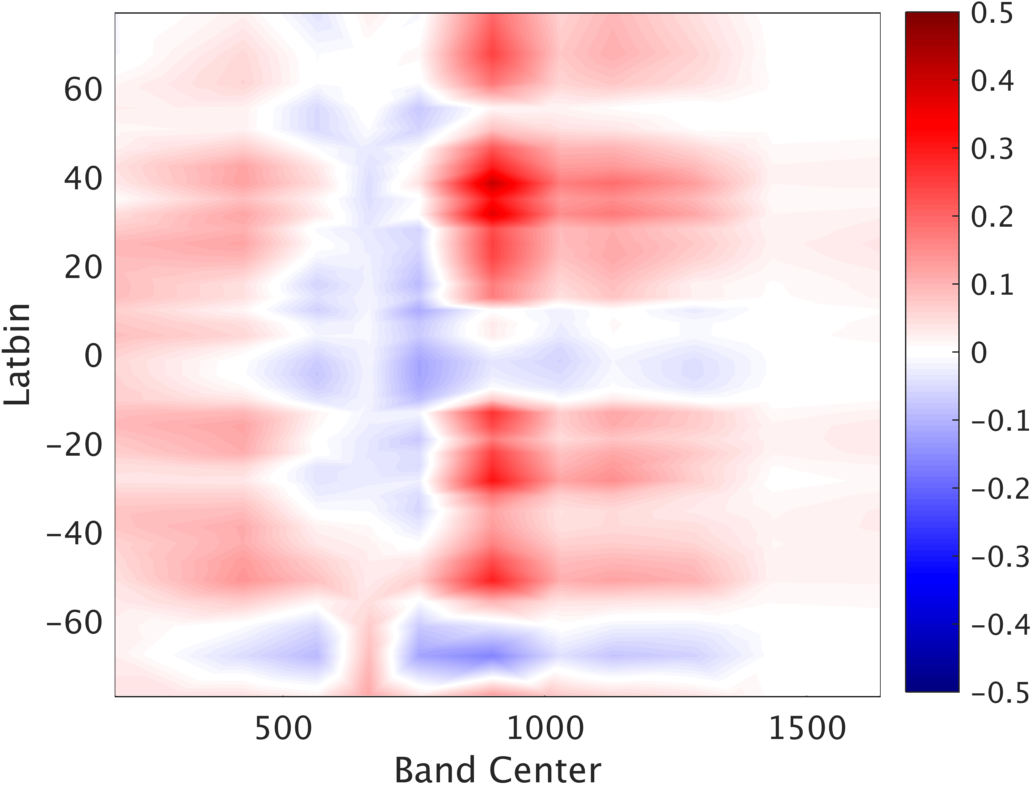
\includegraphics[width=0.625\linewidth]{Figs/umbc_vs_band_fluxrates.png}
  \end{center}
\end{frame}

\begin{frame}
  \frametitle{Breakdown of changes 1 : OLR}
%  \begin{center}
%    \noindent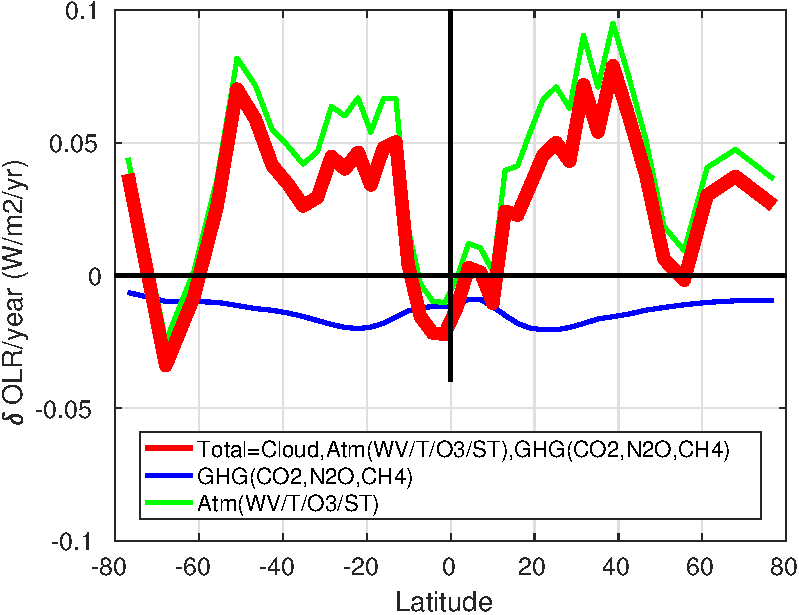
\includegraphics[width=0.625\linewidth]{Figs/umbc_total_vs_atm_vs_GHG.pdf}
%  \end{center}
  \hspace{0.50in} Clouds/Atmos/GHG  \hspace{1.5in} Ind. Gases \\
  \begin{center}
    \dlandgraph{0.48}{Figs/umbc_total_vs_atm_vs_GHG.png}{Figs/umbc_total_vs_atm_vs_GHG2.png}
  \end{center}
 Errorbars : TBD for next AIRS STM \newline
 Total = Cloud/Atm/GHG where \newline
 \textcolor{blue}{Cloud=}Water+Ice, \textcolor{blue}{GHG=}\cd,\methane,\nitrous, \textcolor{blue}{Atm=}SurfTemp,T,\water,\ozone
\end{frame}

\begin{frame}
  \frametitle{Breakdown of changes 2A : Spectral Flux}
%  \begin{center}
%    \noindent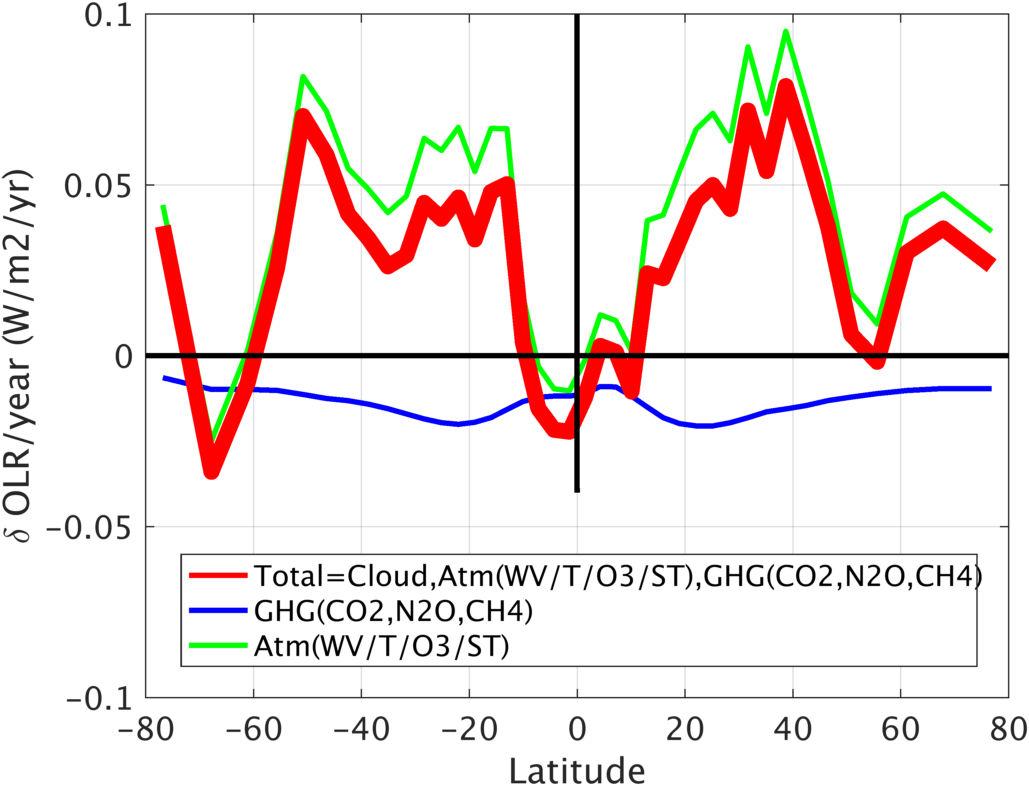
\includegraphics[width=0.625\linewidth]{Figs/umbc_total_vs_atm_vs_GHG.png}
%  \end{center}
  \hspace{0.50in} WV  \hspace{1.5in} CO2 \\
  \begin{center}
    \dlandgraph{0.48}{Figs/umbc_wvonly_spectralfluxchange.png}{Figs/umbc_co2only_spectralfluxchange.png}
  \end{center}
 Errorbars : TBD for next AIRS STM
\end{frame}

\begin{frame}
  \frametitle{Breakdown of changes 2B : Spectral Flux}
%  \begin{center}
%    \noindent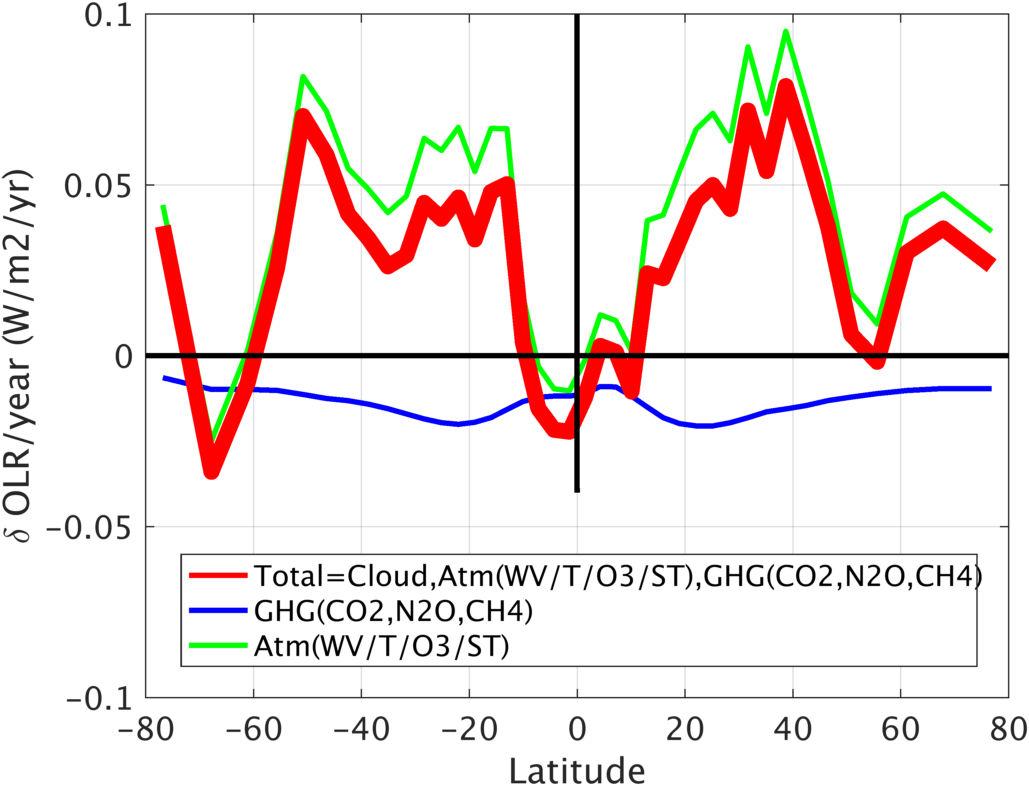
\includegraphics[width=0.625\linewidth]{Figs/umbc_total_vs_atm_vs_GHG.png}
%  \end{center}
  \hspace{0.50in} Surf. Temp  \hspace{1.5in} Atm. Temp \\
  \begin{center}
    \dlandgraph{0.48}{Figs/umbc_STonly_spectralfluxchange.png}{Figs/umbc_Tonly_spectralfluxchange.png}
  \end{center}
 Errorbars : TBD for next AIRS STM
\end{frame}
% ---------------------------------------------------------------------
% ---------------------------------------------------------------------
\section{Conclusions}
% ---------------------------------------------------------------------
% ---------------------------------------------------------------------
\begin{frame}
  \frametitle{Conclusions}
  \begin{itemize}
  \item RRTM allows us to dissect changes to OLR according to spectral region
  \item This gives us a different way to study climate trends
  \item TwoSlab fluxes "not too bad"!
  \item ERA TwoSlab cloud trends $\rightarrow$ RRTM : large change in cirrus fraction
        produces unrealistically large OLR changes
  \item UMBC Spectral Rates $\rightarrow$ Thermodynamic+Cloud rates \textcolor{red}{good agreement
        with OLR rates from CERES}
  \item Much improved flux constraints using our retrievals on 15 years AIRS spectral rates
  \item To do list : try MRO clouds in RRTM ....
  \end{itemize}
\end{frame}
% ---------------------------------------------------------------------
% ---------------------------------------------------------------------

% ---------------------------------------------------------------------
% ---------------------------------------------------------------------
\section{Extra Slides : Flux Changes by RRTM bands : ERA clouds}
% ---------------------------------------------------------------------
% ---------------------------------------------------------------------
\begin{frame}
  \frametitle{Flux Changes by RRTM bands}
  RED means MORE flux (W/m2) in 2017/2018 \newline
  \hspace{0.50in} Clear Sky  \hspace{1.75in} All Sky \\
  \begin{center}
    \dlandgraph{0.48}{Figs/spectral_deltaolr_vs_lat_thermo_gases.png}{Figs/spectral_deltaolr_vs_lat_thermo_gases_clouds.png}
  \end{center}

  \begin{small}
    \begin{itemize}
    \item \textcolor{red}{fix all this, loooks wrong}
    \item LH panel, can see in 15 um band the change is red
    \item LH panel, can see more clr sky flux coming out in Southern Polar Regions in thermal window
    \item RH panel, more flux coming out in tropical window region in 2002
    \item RH panel, can see topical WV region had more flux emitted in 2002
    \end{itemize}
  \end{small}
\end{frame}


\end{document}
% ---------------------------------------------------------------------
% ---------------------------------------------------------------------

% ---------------------------------------------------------------------
% ---------------------------------------------------------------------
\section{Time series}
% ---------------------------------------------------------------------
% ---------------------------------------------------------------------
\begin{frame}
  \frametitle{Calculated Time Series (using ERA)}
  Monthly W/m2 from 2002/09 to 2017/08 \newline
  \hspace{0.50in} No Clouds  \hspace{1.75in} TwoSlab Clouds \\
  \begin{center}
    \dlandgraph{0.48}{Figs/olr_lat_time_nocloud.pdf}{Figs//olr_lat_time_cloud.pdf}
  \end{center}
\end{frame}
% ---------------------------------------------------------------------
%\begin{frame}
%  \frametitle{Greenhouse Effect}
%  Monthly W/m2 from 2002/09 to 2017/08 \newline
%  We know monthly averaged surface temperatures so we know power
%  emitted at surface, so we can compute GH effect (with clouds is
%  larger than without clouds) \newline 
%  \hspace{0.50in} GHG only \hspace{1.75in} GHG + CLouds \\
%  \begin{center}
%    \dlandgraph{0.48}{Figs/ghgeffect_delta_sb_olr_lat_time_nocloud.pdf}{Figs/ghgNcloudeffect_delta_sb_olr_lat_time.pdf}
%  \end{center}
%\end{frame}
% ---------------------------------------------------------------------
\begin{frame}
  \frametitle{Comparisons to CERES}
  CERES OLR - ERA TwoSlab OLR  (W/m2)
  \begin{center}
    \noindent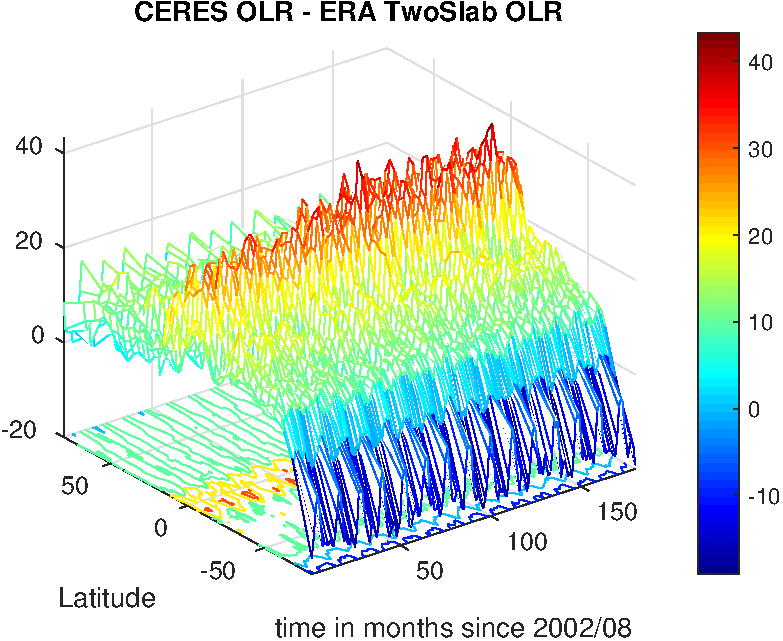
\includegraphics[width=0.625\linewidth]{Figs/ceresVSghgNcloudeffect_lat_time.pdf}
  \end{center}
  So clearly ERA clouds $\rightarrow$ TwoSlab/Fluxes shows much larger changes in OLR than observed!
\end{frame}

%%%%%%%%%%%%%%%%%%%%%%%%%%%%%%%%%%%%%%%%%%%%%%%%%%%%%%%%%%%%%%%%%%%%%%%%
